\section{lg\-Event Class Reference}
\label{classlgEvent}\index{lgEvent@{lgEvent}}
A {\bf lg\-Object} with duration and time-position.  


{\tt \#include $<$lgevent.h$>$}

Inheritance diagram for lg\-Event::\begin{figure}[H]
\begin{center}
\leavevmode
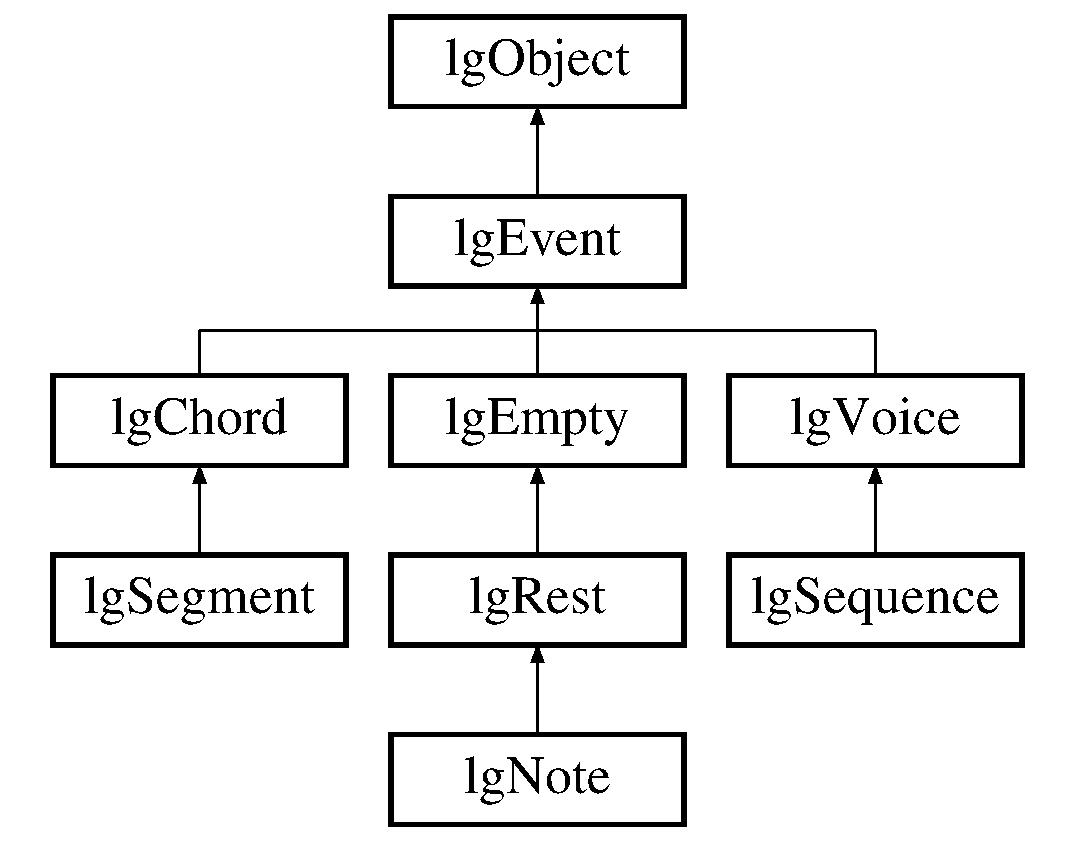
\includegraphics[height=5cm]{classlgEvent}
\end{center}
\end{figure}
\subsection*{Public Member Functions}
\begin{CompactItemize}
\item 
{\bf lg\-Event} (long int dur\-Num, long int dur\-Denom, int cdots, long int pos\-Num, long int pos\-Denom)
\item 
virtual string {\bf to\-String} ({\bf lg\-Voice} $\ast$calling\-Seq=NULL)
\begin{CompactList}\small\item\em lg\-Event returns only the duration as a string \item\end{CompactList}\item 
virtual lg\-Frac {\bf duration} (void)
\begin{CompactList}\small\item\em duration of event including c\-Dot info! \item\end{CompactList}\item 
virtual lg\-Frac {\bf head\-Duration} (void)
\begin{CompactList}\small\item\em return only explicite written duration without dots, is zero for lg\-Voice! \item\end{CompactList}\item 
int {\bf c\-Dots} (void)
\begin{CompactList}\small\item\em number of written dots \item\end{CompactList}\item 
virtual void {\bf set\-Duration} ({\bf lg\-Duration} dur, int dots=0)
\begin{CompactList}\small\item\em set the duration \item\end{CompactList}\item 
virtual lg\-Frac {\bf pos} (void)
\begin{CompactList}\small\item\em absolute time position. needs to be updated if previous events were inserted or deleted! \item\end{CompactList}\item 
virtual void {\bf set\-Pos} (const lg\-Frac \&pos)
\begin{CompactList}\small\item\em be carefull that list is consistent! \item\end{CompactList}\item 
virtual void {\bf write} (FILE $\ast$out, {\bf lg\-Voice} $\ast$call\-Seq)
\begin{CompactList}\small\item\em write own data AND all tags starting in call\-Seq in (this-$>$pos...next-$>$pos] \item\end{CompactList}\item 
{\bf lg\-Note} $\ast$ {\bf next\-Note} (void)
\begin{CompactList}\small\item\em skip all rests, etc. \item\end{CompactList}\end{CompactItemize}
\subsection*{Protected Member Functions}
\begin{CompactItemize}
\item 
virtual void {\bf write\-V} (FILE $\ast$out)
\end{CompactItemize}
\subsection*{Private Attributes}
\begin{CompactItemize}
\item 
{\bf lg\-Duration} {\bf pos\-I}
\begin{CompactList}\small\item\em time position of event, events of a voice must not overlap each other! \item\end{CompactList}\item 
{\bf lg\-Duration} {\bf duration\-I}
\begin{CompactList}\small\item\em the \char`\"{}written\char`\"{} duration excluding dots (= duration of notehead)! \item\end{CompactList}\item 
long int {\bf c\-Dots\-I}
\begin{CompactList}\small\item\em the number of dots \item\end{CompactList}\end{CompactItemize}
\subsection*{Friends}
\begin{CompactItemize}
\item 
class {\bf lg\-Voice}
\begin{CompactList}\small\item\em needs access to set\-Next \item\end{CompactList}\item 
class {\bf lg\-Chord}
\begin{CompactList}\small\item\em needs access to set\-Next \item\end{CompactList}\end{CompactItemize}


\subsection{Detailed Description}
A {\bf lg\-Object} with duration and time-position. 



\subsection{Constructor \& Destructor Documentation}
\index{lgEvent@{lg\-Event}!lgEvent@{lgEvent}}
\index{lgEvent@{lgEvent}!lgEvent@{lg\-Event}}
\subsubsection{\setlength{\rightskip}{0pt plus 5cm}lg\-Event::lg\-Event (long int {\em dur\-Num}, long int {\em dur\-Denom}, int {\em cdots}, long int {\em pos\-Num}, long int {\em pos\-Denom})}\label{classlgEvent_a0}


close range\-Stack gives the number of \char`\"{})\char`\"{} which should be placed after \char`\"{}this\char`\"{} in the .gmn out. If any tag or note is added/removed to/from the tag/note list, close\-Range needs to be updated -$>$ see {\bf lg\-Voice} 

\subsection{Member Function Documentation}
\index{lgEvent@{lg\-Event}!cDots@{cDots}}
\index{cDots@{cDots}!lgEvent@{lg\-Event}}
\subsubsection{\setlength{\rightskip}{0pt plus 5cm}int lg\-Event::c\-Dots (void)\hspace{0.3cm}{\tt  [inline]}}\label{classlgEvent_a4}


number of written dots 

\index{lgEvent@{lg\-Event}!duration@{duration}}
\index{duration@{duration}!lgEvent@{lg\-Event}}
\subsubsection{\setlength{\rightskip}{0pt plus 5cm}{\bf lg\-Duration} lg\-Event::duration (void)\hspace{0.3cm}{\tt  [virtual]}}\label{classlgEvent_a2}


duration of event including c\-Dot info! 



Reimplemented in {\bf lg\-Voice} {\rm (p.\,\pageref{classlgVoice_a22})}.\index{lgEvent@{lg\-Event}!headDuration@{headDuration}}
\index{headDuration@{headDuration}!lgEvent@{lg\-Event}}
\subsubsection{\setlength{\rightskip}{0pt plus 5cm}virtual lg\-Frac lg\-Event::head\-Duration (void)\hspace{0.3cm}{\tt  [inline, virtual]}}\label{classlgEvent_a3}


return only explicite written duration without dots, is zero for lg\-Voice! 

\index{lgEvent@{lg\-Event}!nextNote@{nextNote}}
\index{nextNote@{nextNote}!lgEvent@{lg\-Event}}
\subsubsection{\setlength{\rightskip}{0pt plus 5cm}{\bf lg\-Note} $\ast$ lg\-Event::next\-Note (void)}\label{classlgEvent_a9}


skip all rests, etc. 

\index{lgEvent@{lg\-Event}!pos@{pos}}
\index{pos@{pos}!lgEvent@{lg\-Event}}
\subsubsection{\setlength{\rightskip}{0pt plus 5cm}virtual lg\-Frac lg\-Event::pos (void)\hspace{0.3cm}{\tt  [inline, virtual]}}\label{classlgEvent_a6}


absolute time position. needs to be updated if previous events were inserted or deleted! 



Reimplemented from {\bf lg\-Object} {\rm (p.\,\pageref{classlgObject_a5})}.\index{lgEvent@{lg\-Event}!setDuration@{setDuration}}
\index{setDuration@{setDuration}!lgEvent@{lg\-Event}}
\subsubsection{\setlength{\rightskip}{0pt plus 5cm}virtual void lg\-Event::set\-Duration ({\bf lg\-Duration} {\em dur}, int {\em dots} = 0)\hspace{0.3cm}{\tt  [inline, virtual]}}\label{classlgEvent_a5}


set the duration 

\index{lgEvent@{lg\-Event}!setPos@{setPos}}
\index{setPos@{setPos}!lgEvent@{lg\-Event}}
\subsubsection{\setlength{\rightskip}{0pt plus 5cm}virtual void lg\-Event::set\-Pos (const lg\-Frac \& {\em pos})\hspace{0.3cm}{\tt  [inline, virtual]}}\label{classlgEvent_a7}


be carefull that list is consistent! 

\index{lgEvent@{lg\-Event}!toString@{toString}}
\index{toString@{toString}!lgEvent@{lg\-Event}}
\subsubsection{\setlength{\rightskip}{0pt plus 5cm}string lg\-Event::to\-String ({\bf lg\-Voice} $\ast$ {\em calling\-Seq} = NULL)\hspace{0.3cm}{\tt  [virtual]}}\label{classlgEvent_a1}


lg\-Event returns only the duration as a string 



Reimplemented from {\bf lg\-Object} {\rm (p.\,\pageref{classlgObject_a3})}.

Reimplemented in {\bf lg\-Chord} {\rm (p.\,\pageref{classlgChord_a6})}, {\bf lg\-Empty} {\rm (p.\,\pageref{classlgEmpty_a0})}, {\bf lg\-Note} {\rm (p.\,\pageref{classlgNote_a0})}, {\bf lg\-Rest} {\rm (p.\,\pageref{classlgRest_a0})}, {\bf lg\-Segment} {\rm (p.\,\pageref{classlgSegment_a21})}, {\bf lg\-Sequence} {\rm (p.\,\pageref{classlgSequence_a0})}, and {\bf lg\-Voice} {\rm (p.\,\pageref{classlgVoice_a20})}.\index{lgEvent@{lg\-Event}!write@{write}}
\index{write@{write}!lgEvent@{lg\-Event}}
\subsubsection{\setlength{\rightskip}{0pt plus 5cm}void lg\-Event::write (FILE $\ast$ {\em out}, {\bf lg\-Voice} $\ast$ {\em call\-Seq})\hspace{0.3cm}{\tt  [virtual]}}\label{classlgEvent_a8}


write own data AND all tags starting in call\-Seq in (this-$>$pos...next-$>$pos] 



Reimplemented from {\bf lg\-Object} {\rm (p.\,\pageref{classlgObject_a4})}.

Reimplemented in {\bf lg\-Chord} {\rm (p.\,\pageref{classlgChord_a7})}, {\bf lg\-Segment} {\rm (p.\,\pageref{classlgSegment_a22})}, and {\bf lg\-Voice} {\rm (p.\,\pageref{classlgVoice_a21})}.\index{lgEvent@{lg\-Event}!writeV@{writeV}}
\index{writeV@{writeV}!lgEvent@{lg\-Event}}
\subsubsection{\setlength{\rightskip}{0pt plus 5cm}virtual void lg\-Event::write\-V (FILE $\ast$ {\em out})\hspace{0.3cm}{\tt  [inline, protected, virtual]}}\label{classlgEvent_b0}


should be overwritten in derived classes write class spec values (pitch, \_\-, ..) 

\subsection{Friends And Related Function Documentation}
\index{lgEvent@{lg\-Event}!lgChord@{lgChord}}
\index{lgChord@{lgChord}!lgEvent@{lg\-Event}}
\subsubsection{\setlength{\rightskip}{0pt plus 5cm}friend class {\bf lg\-Chord}\hspace{0.3cm}{\tt  [friend]}}\label{classlgEvent_n1}


needs access to set\-Next 



Reimplemented from {\bf lg\-Object} {\rm (p.\,\pageref{classlgObject_n5})}.

Reimplemented in {\bf lg\-Voice} {\rm (p.\,\pageref{classlgVoice_n0})}.\index{lgEvent@{lg\-Event}!lgVoice@{lgVoice}}
\index{lgVoice@{lgVoice}!lgEvent@{lg\-Event}}
\subsubsection{\setlength{\rightskip}{0pt plus 5cm}friend class {\bf lg\-Voice}\hspace{0.3cm}{\tt  [friend]}}\label{classlgEvent_n0}


needs access to set\-Next 



Reimplemented from {\bf lg\-Object} {\rm (p.\,\pageref{classlgObject_n1})}.

\subsection{Member Data Documentation}
\index{lgEvent@{lg\-Event}!cDotsI@{cDotsI}}
\index{cDotsI@{cDotsI}!lgEvent@{lg\-Event}}
\subsubsection{\setlength{\rightskip}{0pt plus 5cm}long int {\bf lg\-Event::c\-Dots\-I}\hspace{0.3cm}{\tt  [private]}}\label{classlgEvent_r2}


the number of dots 

\index{lgEvent@{lg\-Event}!durationI@{durationI}}
\index{durationI@{durationI}!lgEvent@{lg\-Event}}
\subsubsection{\setlength{\rightskip}{0pt plus 5cm}{\bf lg\-Duration} {\bf lg\-Event::duration\-I}\hspace{0.3cm}{\tt  [private]}}\label{classlgEvent_r1}


the \char`\"{}written\char`\"{} duration excluding dots (= duration of notehead)! 

\index{lgEvent@{lg\-Event}!posI@{posI}}
\index{posI@{posI}!lgEvent@{lg\-Event}}
\subsubsection{\setlength{\rightskip}{0pt plus 5cm}{\bf lg\-Duration} {\bf lg\-Event::pos\-I}\hspace{0.3cm}{\tt  [private]}}\label{classlgEvent_r0}


time position of event, events of a voice must not overlap each other! 



The documentation for this class was generated from the following files:\begin{CompactItemize}
\item 
{\bf lgevent.h}\item 
{\bf lgevent.cpp}\end{CompactItemize}
